\subsection{変数選択への介入}



% どういうランダム関数を使って書き換えたか
% 介入ファイルのフォーマット
% どの順番で変数を書き換えたのか



% 概要
準備の部分で述べたように、minisatは各変数にスコアを割り当てており、変数選択を行う際にこのスコアが一番高い変数を選ぶ仕組みになっている。
この変数のスコアを変更するように介入を行なった。
minisatの変数選択に介入する際には
\begin{itemize}
	\item 介入のタイミング(何回目の変数選択で介入を行うか)
	\item ランダムで書き換えることを指定する値、または一度行なった介入を再現するためのシード値
\end{itemize}
の2つを指定することで変数選択に介入を行えるようにminisatを改造した。
複数回介入を行う際にはこの2つの値を並べることで複数回の介入を行うことができる。
2つ目の要素として一度行なった介入を再現できるようにしている理由は、
後述する遺伝アルゴリズムと組み合わせる際には一度行なった介入を再度行わなければならない可能性があるためである。
つまり一度書き換えた各変数のスコアを再現しなければならないということである。

% 介入の概要
まずは介入におけるスコアの書き換え方について説明する。
この介入はminisatが変数選択を行う前に全ての変数に対してそのスコアを0以上1未満のランダムな値で置き換える。
この書き換えを行うために2つの関数を定義した。

% 介入における1つ目の関数
1つ目は主にどの書き換えを行うかを判断する関数rewriteActivityである。
この関数では$i$回目の変数選択における変数の書き換えがどのような書き換えであるかを、
if文を用いて判断してその指定した書き換えに対応した処理を行う。
どの書き換えを行うかの識別方法については一番目の介入からn番目の介入までの各介入における書き換え方の情報が格納されている配列のメンバ変数usr\_rewritesをこの識別に使用する。
この配列は整数型を要素とする配列となっており、各整数に対応してどのような書き換えを行うかを決めている。
今回は、なにもしない場合、ランダムに置き換える場合、1度行ったランダムな書き換えを再度再現する場合の3種類を定義し、
それぞれ0,1,2の値を割り当てている。
メンバ変数next\_interventionには今行おうとしている介入が何番目の介入になっているかを表す整数型の変数であり、
これと組み合わせることで今行おうとしている書き換えがどのような書き換えであるかを判断することができる。
それぞれの書き換え方に応じた処理については、何もしない場合は何の処理も行わず、
他2つについては2つ目で説明する新しい関数randomActivityを呼び出して処理を行う。
新しくランダムに書き換える場合と1度行った書き換えを再現するかの判断は関数randomActivityの中でも判断している。
このプログラムは若干冗長なプログラムになっているが、別の書き換えを追加する際に追加しやすいようにこのような形のプログラムにしている。
今回はランダムな書き換えがメインであり、基本的に書き換えを行わない介入は介入をしないことと同じ意味なので、if文による分岐を行わず関数randomActivityを呼び出すことでも同様の書き換えを行うことができる。
別の書き換えを行いたい場合はその書き換えに対して0,1,2以外の値を割り当てて、
その値が格納されていた場合に別の書き換えを行う処理を新しい条件分岐として追加することで実装することができる。
\begin{lstlisting}[caption=関数rewriteActivity(core/Solver.cc)]
	// 指定したモードに応じた関数を呼び出してアクティビティを書き換える
	void Solver::rewriteActivity() {
    	// 何もしない場合
    	if        (usr_rewrites[next_intervention] == 0) {
		// ランダムに書き換える場合
    	} else if (usr_rewrites[next_intervention] == 1) {
    	    randomActivity();
		// ランダムに書き換える場合(以前行なった書き換えをもう一度再現する)
    	} else if (usr_rewrites[next_intervention] == 2) {
    	    randomActivity();
    	} else {
    	    cout << "error(rewriteActivity):書き換えのモードが存在しません usr_rewrites[next_intervention] = " << usr_rewrites[next_intervention] << endl;
    	    exit(1);
    	}
	}
\end{lstlisting}

% 介入における2つ目の関数
2つ目はランダムに変数のスコアの書き換えを行うrandomActivityである。
この関数は0番目の変数から順にそのスコア(アクティビティ)を0以上1未満のランダムな値で書き換える。
ランダムな値を生成する方法として今回はメルセンヌ・ツイスター法による疑似乱数生成機mt19937を使用する。
各変数のスコアはmt19937とコンストラクタuniform\_real\_distributionを組み合わせて、0以上1未満の範囲で等確率に生成された値になる。
この各変数のスコアの書き換えを0番目の変数からn番目の変数まで順に行う。
その後このスコアにおいて一番値が大きい変数が選ばれるように関数rebuildOrderHeap()を呼び出す。
minisatは変数選択における変数の選び方として、ヒープ構造を使用してスコアが一番大きい変数を選ぶ方法を使っている。
そのため変数のスコアが変わった際にはヒープ構造を作り直す必要があり、このヒープ構造の作り直しのために関数rebuildOrderHeap()を呼び出している。
一度行った書き換えを再度行う方法としては、シード値を扱うことでこの方法を再現した。
各変数のスコアを保存しておいて再度書き換えを行う際にそのスコアを受け取って書き換えることでも再現可能だが、
変数の数が多い場合に保存するデータ量が莫大なものになってしまうためシード値で扱う方法を使用した。
各変数のスコアを書き換える前のシード値を保存しておいて、
実際に書き換えの再現を行う際は書き換えを行う前にそのシード値で現在のシード値が格納されている変数seedを更新する。
シード値は真の乱数生成を行うことができるrandom\_deviceを使用する。
真の乱数生成は疑似乱数生成に比べて処理速度が遅いので, 疑似乱数生成器のシード生成するためにだけ使用する。
また、このシード値はファイルdelivery\_data.txtにその時の変数選択数と一緒に保存される。
\begin{lstlisting}[caption=関数randomActivity(core/Solver.cc)]
	// ランダムにアクティビティを書き換える
	void Solver::randomActivity() {

    	random_device seed_gen;
    	unsigned int seed = seed_gen();

		// 書き換えの再現を行う場合はその時のシード値を読み込む
    	if (usr_rewrites[next_intervention] == 2) {
    	    seed = usr_seeds[next_intervention];
    	}

		// 今回の書き換えにおけるシード値を出力
    	ofstream outputfile("delivery_data.txt", ios::app);
    	outputfile << decisions << " " << seed << endl;
    	outputfile.close();

    	// 擬似乱数の生成
    	mt19937 mt(seed); // メルセンヌ・ツイスタ

    	// 各アクティビティの書き換え
    	uniform_real_distribution d(0.0, 1.0);
    	for (int i=0; i<activity.size(); i++) {
    	    activity[i] = d(mt);
    	}
    
    	// リビルド
    	rebuildOrderHeap();

	}
\end{lstlisting}

% タイミングの設定
介入のタイミングは何回目の変数選択数で介入を行うかで指定できるようにした。
minisatはメンバ変数decisionsを所持しておりこの変数には現在の変数選択回数が格納されているため、
このメンバ変数が指定した介入のタイミングと一致した際に介入を行うようにしている。
また、このメンバ変数は探索を行う関数searchの中で変数選択を行う関数pickBranchLitを呼び出す前に1増加するようになっている。

% 全部を組み合わせる(上2つの関数の場所など)
上記の2つの関数が指定したタイミングにおいて実行されるように既存の関数に対して変更を行なった。
この関数は変数選択を行う関数pickBranchLitであり、
ヒープ構造を利用して未割当変数の中でスコアが一番大きな変数を返す。
介入のタイミングであるかどうかは変数選択を行う度if文によってチェックを行い、スコアの書き換えを行う。
各介入のタイミングの情報は新しく定義した配列のメンバ変数usr\_interventionsに格納されており、
次の介入が何番目の介入であるかを表す新しく定義した整数型のメンバ変数next\_interventionと組み合わせることで、
次の介入のタイミングを確認することができる。
関数rewriteActivityの呼び出しによって介入が終了した後、次の介入の情報を確認できるようにメンバ変数next\_interventionの値を1増加させる。
\begin{lstlisting}[caption=関数pickBranchLitの変更による介入の追加(core/Solver.cc), firstnumber=249]
	Lit Solver::pickBranchLit()
	{
    	Var next = var_Undef;

    	// Random decision:
    	if (drand(random_seed) < random_var_freq && !order_heap.empty()){
        	next = order_heap[irand(random_seed,order_heap.size())];
        	if (value(next) == l_Undef && decision[next])
            	rnd_decisions++; }
		
		// 追記開始
		// ユーザが介入する場合
		assert(decisions>0);    // usr_interventionsの最後は-1だからそこを見ている限りはnext_interventionは増えない(エラーに行かない)
		if (usr_interventions[next_intervention] == decisions) {
			
			// アクティビティを変更する
			rewriteActivity();
			
			// 次の介入情報を見る
			next_intervention++;
			
		}
		// 追記終了

    	// Activity based decision:
    	while (next == var_Undef || value(next) != l_Undef || !decision[next])
        	if (order_heap.empty()){
        	    next = var_Undef;
        	    break;
        	}else
            	next = order_heap.removeMin();

    	// Choose polarity based on different polarity modes (global or per-variable):
    	if (next == var_Undef)
    	    return lit_Undef;
    	else if (user_pol[next] != l_Undef)
    	    return mkLit(next, user_pol[next] == l_True);
    	else if (rnd_pol)
    	    return mkLit(next, drand(random_seed) < 0.5);
    	else
    	    return mkLit(next, polarity[next]);
	}
\end{lstlisting}



% 介入ファイルのフォーマット
介入ファイルの読み込み方法について説明する前に今回使用する介入ファイルのフォーマットについて説明を行う。
介入ファイルは最初の行が介入の回数を表す情報になっており、その後ろの行では1回目の介入から最後の介入についてどのような介入を行うかの情報が書き込まれている。
各介入の情報は2行の文字列から構成されており、最初の行が介入のタイミング(何回目の変数選択で介入を行うか)で、次の行がどのような介入を行うかを表している。
介入のタイミングについては次の介入におけるタイミングが前の介入のタイミングより大きくなることを予測しており、
万が一介入ファイルが($i$回目における介入のタイミング)$\geq$($i+1$回目における介入のタイミング)となっていた場合は、
$i$回目までの介入を行い、それ以降の介入は行わない処理になっている。
また全ての行が「タグ 値 ...」の形をしている。
タグは1文字で表現されており、介入の回数を表すタグi、介入のタイミングを表すタグt、変数のスコアの書き換え方法を表すタグaの3種類が存在する。
1つ目の介入の回数を表すタグiで始まる行は後ろに0以上の整数の値を1つ取り、この値には介入の回数が書き込まれる。
この介入の回数だけ後ろに各介入を表す情報が書き込まれる。
2つ目の介入のタイミングを表すタグtで始まる行は後ろに自然数の値を1つ取り、この値には何回目の変数選択で介入を行うかが書き込まれる。
3つ目の変数のスコアの書き換え方を表すタグaで始まる行は後ろに1つの値もしくは2つの値を取る。
後ろの値は文字列の値でスコアの書き換え方法を表しており、
ランダムに介入を行う``Random''もしくは1度行った介入をもう一度行う``Random\_reproduction''のどちらかをとる。
値が``Random\_reproduction''である場合はさらにその後ろに整数の値をもう1つとり、
この値には再現したいスコアの書き換え方を表すシード値が書き込まれる。
このシード値は関数randomActivityにおいて変数のスコアを書き換える前に設定したシード値である。
図\ref{fig:介入ファイルの例}に表示される図は介入ファイルの1例を表したものである。
この介入ファイルは3回の介入が存在し、それぞれ5119回目、8802回目、13595回目の変数選択において介入がおこなわれる。
1回目と3回目の介入においては変数のスコアをランダムに書き換え、2回目の介入においてはシード値が754015860であった際の変数のスコアの書き換え方を再現する。
\begin{figure}[t]
	\fbox{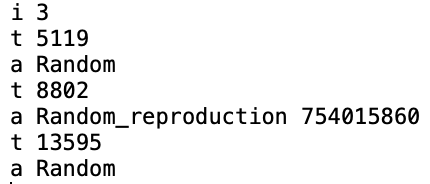
\includegraphics[width=5cm]{figures/example-intervention-file.png}}
   	\caption{介入ファイルの例}
	\label{fig:介入ファイルの例}
\end{figure}

% ファイルの読み込みによる変数への値格納を行う関数
続いて介入ファイルをどのように読み込んでどの変数にその情報を格納したかについて説明する。
介入ファイルを読み込む処理を行う関数として関数read\_interventionを作成した。
この関数は各介入における介入のタイミングを格納する配列のメンバ変数と変数のスコアの書き換え方を格納する配列のメンバ変数と
書き換えの再現に用いられるシード値を格納する配列のメンバ変数に対して介入の情報を格納する。
また、介入のタイミングを格納する配列については全ての介入の情報を読み終わった後にそれ以降は介入が行われないことを表す値を追加する。
この3つのメンバ変数はそれぞれusr\_interventions, usr\_rewrites, usr\_seedsという変数で、
全て今回の実装において新しく定義した変数であり、各要素が整数となっている配列である。
ファイルを読み込むためにクラスifstreamを使用し、演算子$>>$を使って1つずつ値を読み取っていく。
最初に1行目にある介入の情報を読み取ることで介入の回数を取得し、その回数だけ介入の情報を読み取っていく。
介入の情報はタイミング、スコアの書き換え方の順で情報を読み取りそれぞれメンバ変数usr\_interventions, usr\_rewritesの最後尾の要素として追加する。
スコアの書き換え方については各文字列に対応した値に変換してから追加する。
シード値の読み取りについてはスコアの書き換え方が1度行なった介入の再現の場合は値をファイルから読み込み、それ以外の場合はダミーのシード値として0を使って
メンバ変数usr\_seedsの最後尾に追加する。
実際にこのusr\_seedsの要素は介入が1度おこなった介入の再現である場合のみ参照されるため、ダミーの値は0以外の値でも問題ない。
介入の情報を全て読み込んだ後はそれ以降介入がないことを表す値$-1$をメンバ変数usr\_interventionsの最後尾に追加する。
この値を追加する理由は介入を行うかどうかを判断する際には、
現在の変数選択数を表すメンバ変数decisionsと次の介入のタイミングが一致しているかどうかで判断しているためである
この変数は0以上であるため、0未満の値をタイミングとして格納しておけばその値を参照している限り、介入は行われない。

\begin{lstlisting}[caption=関数read\_intervention(core/Solver.cc)]
	void SimpSolver::read_intervention(const char* intervention){

    	if (intervention) {
        	// ファイルオープン
        	ifstream intervention_f(intervention);
        	if (!intervention_f) {
            	printf("ファイルオープンに失敗しました%d\n", intervention);
            	exit(1);
        	}

        	// 介入の回数を読み取る
        	string tag;
        	int n_interventions;
        	intervention_f >> tag;
        	if (tag != "i") {
        	    cerr << "error(read_intervention):タグが異なります(iのはずが" << tag << "です)" << endl;
        	    exit(1);
        	}
        	intervention_f >> n_interventions;

        	// i回目の各情報をソルバー内の情報に加える
        	int tag_value;
        	for (int i=0;i<n_interventions;i++){
            	// タイミング
            	intervention_f >> tag;
            	if (tag != "t") {
                	cerr << "error(read_intervention):タグが異なります(tのはずが" << tag << "です)" << endl;
                	exit(1);
            	}
            	intervention_f >> tag_value;
            	usr_interventions.push(tag_value);
            	// アクティビティの書き換え方
            	string rewrite_mode;
            	intervention_f >> tag;
            	if (tag != "a") {
                	cerr << "error(read_intervention):タグが異なります(aのはずが" << tag << "です)" << endl;
                	exit(1);
            	}
            	intervention_f >> rewrite_mode;
				// 各モードに対応した整数型の値を格納する
            	if        (rewrite_mode == "None") {
            	    usr_rewrites.push(0);
            	} else if (rewrite_mode == "Random") {
            	    usr_rewrites.push(1);
            	} else if (rewrite_mode == "Random_reproduction") {
            	    usr_rewrites.push(2);
            	} else {
            	    cout << "error(rewriteActivity):書き換えのモードが存在しません usr_rewrites[next_intervention] = " << usr_rewrites[next_intervention] << endl;;
            	    exit(1);
            	}
				// 書き換えを再現する場合はそのシード値を受け取る
            	unsigned int seed_to_reproduce = 0;
            	if (rewrite_mode == "Random_reproduction") {
            	    intervention_f >> seed_to_reproduce;
            	}
            	usr_seeds        .push(seed_to_reproduce);
        	}

        	// ファイルクローズ
        	intervention_f.close();

    	}


    	// 想定した介入が終わった後になにもさせないようにするための処理
    	usr_interventions.push(-1);


	}
\end{lstlisting}

% 関数の使用場所
介入ファイルを読み込む処理は関数mainの中において、SimpSolverクラスの変数Sを定義した後に追加した。

% オプションの追加
上記の介入をオプションとして選択できるように、
minisatで定義されているオプションのクラスを使用してオプションの定義を行なった。
minisatにおけるオプションはutil/Options.hにおいてクラスOptionの定義を行い、
そのクラスを継承しブール数型のオプションクラスBoolOptionや文字列型のオプションクラスStringOptionを定義している。
既存のオプションはsimp/main.ccの最初の方に
カテゴリー, オプション名, オプションの詳細, (整数型などの場合は範囲も)を指定して各型のオプションクラスの変数を
宣言をすることで実際にそのオプションが使用された場合にその型に適した値を変数に格納しておき後で参照することができる。
stringOption型でオプション名はinterventionとして変数interventionの宣言を行なった。
これによりオプションで``-intervention=介入ファイル名''を追加することで変数interventionに介入ファイル名を保存できるようになった。
\begin{lstlisting}[caption=介入ファイルの読み込みとオプションの選択をするための関数mainへの変更(core/Solver.cc), firstnumber=66]
    IntOption    cpu_lim("MAIN", "cpu-lim","Limit on CPU time allowed in seconds.\n", 0, IntRange(0, INT32_MAX));
    IntOption    mem_lim("MAIN", "mem-lim","Limit on memory usage in megabytes.\n", 0, IntRange(0, INT32_MAX));
    BoolOption   strictp("MAIN", "strict", "Validate DIMACS header during parsing.", false);
	// 追記開始
	// 介入の情報を入れておくファイル
    StringOption intervention   ("MAIN", "intervention", "If given, get the information for interventin from this file.");
	// 追記終了

    parseOptions(argc, argv, true);
        
    SimpSolver  S;
    double      initial_time = cpuTime();

    if (!pre) S.eliminate(true);

	// 追記開始
	// 介入の情報を読み込む(オプションでファイルを指定していない場合は何も介入をさせない処理を行う)
    S.read_intervention((const char*)intervention);
	// 追記終了
    S.verbosity = verb;
\end{lstlisting}

% メンバ変数の追加

% 変数選択を行う関数の流れ(どの関数が呼ばれてどういう処理をするか)
\begin{comment}
	search()
	-pickBranchLit()
	 -rewriteActivity()(新規)
	  -randomActivity()(新規)
	   -rebuildOrderHeap()
\end{comment}